\chapter{Teorie}
% Druhá kapitola s matematikou \texorpdfstring{$\int\! f(x)\,\mathrm{d}x$}{int f(x) dx} v~názvu
%% matematicke symboly nelze do zalozek v PDF vlozit - proto slouzi prikaz \texorpdfstring{toto se vysazi}{toto se
%% vlozi do zalozek v PDF} - nektere symboly vlozit lze, viz kapitolu 50 v dokumentaci
%% http://mirrors.ctan.org/macros/latex/contrib/hyperref/hyperref.pdf
%% viz take http://orgmode.org/worg/org-symbols.html
%%

%%%%%%%%%%%%%%%%%%%%%%%%%%%%%%%%%%%%%%%%%%%%%%%%%%%%%%%%%%%%%%
%%%%%%%%% UKAZKA OPAKOVANI MATEMATICKYCH SYMBOLU %%%%%%%%%%%%%
% 
% ukázka opakování na řádkovém zlomu ukázka opakování na řádkovém zlomu zlom $c+ a+ b$
% 
% ukázka opakování na řádkovém zlomu ukázka opakování na řádkovém zlomu zl $c- a- b$
% 
% ukázka opakování na řádkovém zlomu ukázka opakování na řádkovém zlomu zlo $c\cdot a\cdot b$
% 
% ukázka opakování na řádkovém zlomu ukázka opakování na řádkovém zlomu zl $c\setminus a\setminus b$
% 
Teoretická část práce seznamuje s konceptem parciálních atomových nábojů a~s metodami jejich výpočtu. Blíže popisuje teoretické základy empirických metod EEM a PEOE, které byly použity v praktické části práce, podobně jako uvedené statistické veličiny.

\section{Parciální atomové náboje}

Parciální atomové náboje jsou reálná čísla, která popisují asymetrické rozložení elek\-tronové hustoty na chemické vazbě \cite{Atkins}. Vznikají v důsledku rozdílných elektronegativit vazebných partnerů. Pokud v chemické vazbě figuruje vysoce elektronegativní atom, pak tento k sobě přitahuje vazebný elektronový pár, čímž se zvyšuje elektronová hustota v~ jeho okolí a dochází ke vzniku parciálního záporného náboje ($\delta$-). V okolí elektropozitivnějšího vazebného partnera se elektronová hustota naopak snižuje a~na atomu dochází ke vzniku parciálního kladného náboje ($\delta$+). 

\bigskip
\begin{figure}[h]
\begin{center}
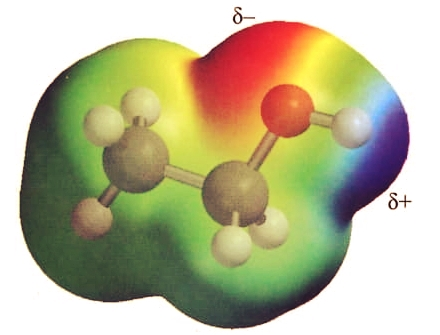
\includegraphics[width=5.5cm]{pictures/partial_atomic_charges_cropped.jpg}
\caption{Parciální atomové náboje v molekule ethanolu. Červená barva značí zvýšenou elektronovou hustotu v blízkosti atomu kyslíku.}
\end{center}
\end{figure}
Koncept parciálních atomových nábojů je pouze teoretický, hodnoty nábojů proto nelze získat pomocí experimentu \cite{Leach}. Jelikož se parciální atomové náboje uplatňují při predikci fyzikálních, chemických a biologických vlastností molekul, bylo pro jejich stanovení vyvinuto množství výpočetních metod. Tyto se dělí na metody kvantově-chemi\-cké a metody empirické. Kvantově-chemické metody představují standardní přístup výpočtu parciálních atomových nábojů,  avšak použití těchto metod může být limitováno jejich velkou časovou náročností. Empirické metody používají v rámci výpočtů parametrizovaná nebo exprimentálně naměřená data a představují tak časově méně náročnou alternativu kvantově-chemického přístupu \cite{Gasteiger:Textbook}. 
% Kvantově-chemické metody poskytují přesnější výsledky, ovšem za cenu vysoké časové náročnosti. Empirické metody dosahují v porovnání s QM metodami velmi dobrých výsledků, a to ve výrazně kratším čase. 
%Žádná z vyvinutých empirických metod však není uznána za všeobecně platnou a jejich použitelnost se hodnotí na základě reprodukovatelnosti výsledků. 

Aplikaci parciálních atomových nábojů lze nalézt ve výpočetní chemii a chemoinformatice, kde slouží k predikci elektrostatických vlastností popisujících reaktivitu molekul. Uplatňují se v molekulových simulacích \cite{molsimul}, ve virtuálním screeningu \cite{virtscreen}, při hledání vazebných míst proteinů nebo při návrhu farmakoforů \cite{farmak}. Prokázaly se jako platné deskriptory v QSAR a QSPR modelech \cite{Ghaf:QSAR, QSPR2}. V anorganické chemii se uplatňují při popisu toku elektronů v bateriích a katalyzátorech \cite{innorg}. 

%%%%%%%%%%%%%%% QC METODY %%%%%%%%%%%%%%%%%%%%%%%%%%%%%
\section{Kvantově-chemické metody}
V této podkapitole je popsán teoretický aparát kvantové mechaniky, na kterém jsou založeny kvantově-chemické metody, které lze použít pro výpočet parciálních atomových nábojů. Tyto metody jsou dále popsány. 

\subsection{Základy kvantové mechaniky}
%Již na konci 19. století došli vědci k poznání, že klasická newtonovská mechanika není vhodná pro popis pohybu mikročástic (např. elektronů). Z toho důvodu došlo ve 20. letech 20. století k rozvoji kvantové mechaniky. 
Kvantová mechanika se rozvinula ve 20. letech 20. století v reakci na newtonovskou mechaniku, jejíž aparát již nepostačoval pro popis mikrosvěta.  Základním principem QM je vlnově-korpuskulární dualismus, který mikročástici připisuje jak charakteristiky hmoty (hybnost), tak charakteristiky elektromagnetické vlny šířící se prostorem.
Vlna, popisující částici, je v kvantové mechanice reprezentována matematickou funkcí $\Psi$, tzv. vlnovou funkcí. Tato funkce popisuje dynamický stav částice a nese informaci o výskytu částice v prostoru \cite{Cely}. Vlnová funkce elektronu tak popisuje rozložení elektronové hustoty v molekule. 

Základním úkolem kvantové mechaniky je výpočet vlnové funkce systému, z níž lze odvodit elektrostatický potenciál \cite{elstat_pot} nebo termodynamické vlastnosti molekuly \cite{td}. Vlnová funkce je řešením Schrödingerovy rovnice (\textit{Schrödinger's Equation}, SE)
\begin{equation}
    H\Psi = E\Psi
\end{equation}
kde $H$ je operátor hamiltonián a $E$ je energie systému. Hamiltonián působí na vlnovou funkci $\Psi$ a transformuje ji na funkci jinou. Řešením Schrödingerovy rovnice je soubor funkcí, které lze po aplikaci hamiltoniánu zapsat jako součin původní funkce a~skaláru $E$. Takovéto funkce označujeme jako \textit{vlastní funkce} a odpovídající skaláry jako \textit{vlastní hodnoty} operátoru \cite{Volatron}. 
 %Řešení Schrödingerovy rovnice pro daný systém tedy odpovídá hledání dvojic vlastních funkcí a vlastních hodnot operátoru $H$ vyhovujících rovnici xx.
 
 Schrödingerova rovnice je exaktně řešitelná pouze pro vybrané problémy, např. pro atom vodíku. Pro víceelektronové systémy je nutno do výpočtu zavádět velké množství aproximací, z nichž nejznámější je Born-Oppenheimerova aproximace \cite{BO_approx_Pilar}.
 Jejím základním konceptem je oddělení řešení SE pro jádra od řešení rovnice elektronů. Tento postup vychází z předpokladu, že jádra atomů, mnohonásobně těžší než elektrony, se pohybují výrazně pomaleji než elektrony samotné, a jejich polohu lze tedy pro řešení SE elektronů pokládat za fixní. %Řešení Schrödingerovy rovnice se tak rozkládá na řešení popisující elektrony v souboru fixních jader, po němž následuje řešení rovnice zahrnující kinetickou a potenciální energii jader obklopených polem elektronů.
 
\subsection{Úvod do kvantově-chemických metod}
Cílem kvantově-chemických (QC) metod je exaktní popis chemických vlastností systému. Jednou ze zkoumaných vlastností je rozložení elektronové hustoty, které je odvozeno z~vlnové funkce molekuly. Znalost rozložení elektronové hustoty v molekule je klíčovým faktorem pro odvození parciálních atomových nábojů.

Kvantově-chemické metody se dělí na tři hlavní skupiny, a to metody semi-empiric\-ké, metody odvozené od teorie funkcionálu hustoty a metody \textit{ab initio}. \textit{Ab initio} metody (lat. \textit{ab initio} - od počátku) staví výpočty na teoretickém aparátu a Schrödingerovu rovnici řeší exaktně, pouze za použití fyzikálních konstant, z čehož vyplývá jejich velká výpočetní náročnost (výpočty těchto metod škálují až s $n^7$, kde \textit{n} je počet elektronů systému \cite{qc_complexity}). Metody semi-empirické jsou stejně jako metody \textit{ab initio} založeny na řešení SE a pro urychlení výpočtů využívají kromě aproximací také data z experimentu. Metody odvozené z DFT nevycházejí z řešení vlnové fukce, ale své poznatky staví na elektronové hustotě v molekule \cite{Leach, Gasteiger:Textbook, Cramer}. %část výpočtů však parametrizují nebo aproximují na základě experimentálních dat.

Postup kvantově-chemické výpočtů pro popis rozložení elektronové hustoty se typicky skládá z následujících kroků: výběr metody, výběr bázové sady a provedení populační analýzy.

\subsubsection{Příklady kvantově-chemických metod}
Následující příklady popisují Hartree-Fockovu metodu, metody odvozených z teorie funkcionálu hustoty a metody semi-empirické.

\begin{itemize}
    \item \textbf{Hartree-Fockova metoda}
    
    Tato raná \textit{ab initio} metoda řeší SE rozložením původní \textit{n}-elektronové vlnové fun\-kce na~řešení \textit{n} jednoelektronových rovnic. Tyto rovnice jsou určeny předpisem $\hat{F} \chi_i = \varepsilon_i \chi_i$, kde $\hat{F}$ je Fockův operátor (Hartreeho-Fockův hamiltonián) aplikovaný na jednoelektronový orbital $\chi_i$. Metoda pracuje iterativním způsobem, a to až do ustálení výsledných hodnot vlnových funkcí. Tento přístup se označuje termínem selfkonzistentní pole (angl. \textit{self-consistent field}, SCF) \cite{Levine}. 
% ver2 
%Interakce elektronu s ostatními elektrony je tedy aproximována na působení vnějšího elektronového pole na danou částici.
% ver1 
%Jednotlivé jednoelektronové rovnice tedy zahrnují působení vnějšího elektronového pole. 
% PŮVODNÍ TEXT K SCF: Problém řešení víceelektronových systémů nastává při zahrnutí elektronových interakcí do výpočtu. Interakce elektronů molekuly lze řešit pomocí přiblížení metody nezávislých částic (SCF, Self-Consistent Field), která pracuje s modelem elektronu pohybujícím se v průměrném poli ostatních elektronů. Původní problém se tak rozkládá na řešení jednoelektronových rovnic, zahrnující působení vnějšího elektronového pole. Teorii SCF využívá Hartree-Fockova metoda, označována jako HF-SCF. 

    \item \textbf{DFT - Density Functional Theory}
    
    Metody založené na teorii funkcionálu hustoty  nenásledují schéma kvan\-tově-chemických metod, ale své výpočty staví na rozložení elektronové hustoty, ze kterého odvozují energii systému a další vlastnosti molekuly \cite{dft_nmr}. Elektronová hustota je funkcí souřadnic \textit{x}, \textit{y}, \textit{z}. V porovnání s řešením Schrödingerovy rovnice, která pro systém s \textit{n} elektrony obsahuje 4\textit{n} neznámých, je její výpočet výrazně jednodušší. Termín 'funkcionál' je v kontextu DFT chápán jako zobrazení, které zobrazuje funkci, představující elektronovu hustotu, do množiny reálných čísel popisujících energii elektronů \cite{dft}.
 %slozitost elektronu SE: Lewards; Gasteiger; Leach; Levine; citovat články od Peti a Bichiho
% Myšlenka DFT: všecky elektronové vlastnosti se získají z elektronové hustoty (např. energie systému/energie základního stavu - Leach) (Peťa BP). Jednodušší v porovnání s výpočtem vlnové funkce, kde je zahrnut ještě popis elektronu. Leach: Cílem DFT je výpočet elektronové hustoty systému a zní získání celkové energie elektronů (electronic energy).
% Typy používaných funkcionálů: Local Density Aproximation (LDA), Generalized Gradient Aproximation (GGA) a Hybrid Functionals (hybridní funkcionály).

    \item \textbf{Semi-empirické metody}
    
    Semi-empirické metody část výpočtů aproximují a při řešení rovnic aplikují parametry odvozené z experimentálních dat, a to s cílem reprodukovat výsledky \textit{ab intio} výpočtů. Příkladem semi-empirické metody je metoda CNDO (\textit{Complete Neglect of Differential Overlap}) \cite{CNDO}. Metoda zamítá interakce atomových orbitalů lokalizovaných na různých atomech molekuly a pracuje pouze s interakcemi atomových orbitalů stejného typu lokalizovaných na stejném atomu. Tato aproximace byla v metodách navazujících na CNDO (INDO \cite{INDO}, MNDO \cite{MNDO}) rozšířena o interakci orbitalů lokalizovaných na jiných jádrech a interakci volných elektronových párů.
\end{itemize}

%část výpočtů však parametrizují nebo aproximují na základě experimentálních dat.
% Atkins
% integral set to zero = překryvem atomových orbitalů nevzniká molekulový orbital (Atkins český, s. 403)
%- QM ve své době limitovány nedostatečnými výpočetními zdroji, aplikace pouze pro malé molekuly -> SE metody: ve větší míře využití aproximací nebo části výpočtů parametrizují na základě exerimentálních dat, snaží se přiblížit své výsedky QM výpočtům
%- příklady metod: EHT rozšířená Hückelova metoda
%- modernější metody: CNDO (využití SCF teorie pro popis elektronových interakcí), založená na ZDO aproximaci (Zero Differential Overlap) - nejsou brány v potaz překryvy orbitalů odlišného typu, jejich překryv roven nule
%- Atk: CNDO - všechny překryvové integrály popisující čtyři atomové orbitaly lokalizované na různých atomech jsou rovny nule = překryvem daných AO nevzniká MO
%- INDO nahradila CNDO - nahrazení hrubých ZDO aproximací, zahrnutí vzájemných interakcí elektronů přislušících stejnému atomu
%- Další vyvinuté metody: NDDO a z ní odvozená MNDO; dále AM1 nebo PM3

\subsubsection{Bázová sada}
Bázová sada je soubor vlnových funkcí reprezentující atomové orbitaly, jejichž vhodnou lineární kombinací (LCAO) lze následně vyjádřit vlnovou funkci molekuly. %Bázová sada obsahující nejmenší možný počet atomových orbitalů potřebných pro konstrukci molekulových orbitalů se označuje jako \textit{minimální báze}. 
 % STO, GTO: handbook of chemoinf, Gasteiger
Pro popis funkcí reprezentujících atomové orbitaly se používají orbitaly Gaussova typu (GTO). Kombinace několika Gaussových orbitalů přibližuje tzv. Slaterův orbital (STO), který je pro výpočet vlnové funkce molekuly méně vhodný z důvodu složitosti výpočtů. Příkladem bázových sad jsou sady STO-3G, STO-4G či obecně STO-\textit{n}G, kde \textit{n} je počet orbitalů Gaussova typu reprezentujících jeden atomový orbital. Dalšími bázovými sadami jsou např. 6-31G nebo 6-21G* \cite{basis_set}.
%sady 6-31G* či 6-311G.

\subsubsection{Populační analýza}
Pomocí populační analýzy je získáno zastoupení elektronů v molekulových orbitalech (rozložení elektronové hustoty), ze kterého lze odvodit parciální atomové náboje. 

V rámci Mullikenovy populační analýzy (\textit{Mulliken Population Analysis}, MPA) \cite{MPA} není brána v potaz rozdílnost elektronegativit vazebných partnerů a elektronová hustota na vytvořené chemické vazbě je tedy rovnoměrně rozdělena mezi příslušné atomy. Výsledky MPA jsou silně závislé na zvolené kvantově-chemické metodě a na velikosti bázové sady. Nevýhody MPA, zejména nepřesnost výsledků související s rozšiřováním bázové sady, řeší přirozená populační analýza (\textit{Natural Population Analysis}, NPA) \cite{NPA}, pracující s přirozenými atomovými orbitaly. Přirozené atomové orbitaly jsou odvozeny z bázové sady a jsou následně použity pro výpočet ortonormálních přirozených vazebných orbitalů (\textit{Natural bonding orbitals}, NBO). Na základě NBO se poté provadí populační analýza.

Odlišný přístup finálního výpočtu parciálních atomových nábojů představuje metoda \textit{Atoms-in-Molecules} (AIM) \cite{AIM}, která přiřazuje náboje atomům na základě integrace elektronové hustoty přes prostor příslušící danému atomu. 

\section{Empirické metody}
Empirické metody výpočtu parciálních atomových nábojů nevycházejí z řešení vlnové funkce systému, ale definují vlastní postupy výpočtu. Vybrané empirické metody se snaží reprodukovat náboje získané kvantově-chemickými přístupy skrze parametrizaci vůči referenční sadě nábojů, jiné definují parciální atomové náboje vlastním způsobem. Narozdíl od kvantově-chemických metod se metody empirické vyznačují nízkou výpočetní náročností.
%U vybraných empirických metod není cílem reprodukovat hodnoty parciálních atomových nábojů získaných kvanto\-vě-chemickými přístupy, zatímco u jiných je tento cíl prioritou.

Empirické metody se dělí na dvě hlavní skupiny, a to metody pracující s topologií molekuly (popisuje počet a typ vazebných partnerů, násobnost vazeb apod.) a~metody pracující s prostorovým uspořádáním molekuly. Metody zastupující obě uvedené skupiny, jmenovitě metoda PEOE a metoda EEM, jsou popsány v odstavcích níže.

\subsection{PEOE}
Metoda PEOE (\textit{Partial Equalization of Orbital Electronegativity}) je také známá pod jménem autorů jako metoda Gasteiger-Marsili \cite{GM}. V rámci výpočtu neuvažuje 3D strukturu molekuly a pracuje pouze s její topologií. Metoda byla navržena pouze pro systémy obsahující $\sigma$ vazby a nekonjugované $\pi$ vazby, metody odvozené z PEOE však původní metodu výrazně rozšířily, a to např. o aplikaci na halogenované a aromatické sloučeniny \cite{MPEOE_aromatic} nebo o výpočty založené na prostorovém uspořádání molekuly \cite{GDAC}.  
% polypeptidy Kang, Y. K., & Scheraga, H. A. (2008). An Efficient Method for Calculating Atomic Charges of Peptides and Proteins from Electronic Populations. The Journal of Physical Chemistry B, 112(17), 5470–5478. doi:10.1021/jp711484f 

Koncept elektronegativity atomových orbitalů, na němž je metoda PEOE založena, vychází z Mullikenovy definice elektronegativity $\chi_A$ atomu \textit{A}
\begin{equation}
    \chi_A = \frac{1}{2}(I_A + E_A)
\end{equation}
Dle Mullikena je elektronegativita atomu určena hodnotami elektronových afinit $ E_A$ a~ionizačních potenciálů $I_A$ jeho valenčních stavů. PEOE připisuje na základě hodnot $I_A$ a $ E_A$ elektronegativitu každému orbitalu valenčního stavu atomu. Elektronegativita $\chi_{iv}$ orbitalu \textit{iv} na atomu \textit{i}
\begin{equation}
\label{PEOE_elneg}
    \chi_{iv} = a_{iv} + b_{iv}Q_i + c_{iv}Q_i^2
\end{equation}
je ovlivněna náboji ostatních orbitalů a tedy i celkovým nábojem příslušného atomu $Q_i$. Koeficienty $a_{iv}$, $b_{iv}$ a $c_{iv}$ jsou empirické parametry vypočtené z ionizačních potenciálů a elektronových afinit neutrálního, kationtového a aniontového stavu příslušného orbitalu.

Při vzniku vazby dochází vlivem elektronegativity atomů k přesunu elektronů od elektropozitivnějšího atomu směrem k elektronegativnějšímu. Interagují spolu přísluš\-né atomové orbitaly a dochází k částečné ekvalizaci (vyrovnání) jejich nábojů. Metoda PEOE pracuje iterativním způsobem. Množ\-ství přeneseného náboje mezi atomy \textit{A} a \textit{B}, pokud má atom \textit{B} vyšší elektronegativitu, je definováno jako 
\begin{equation}
\label{transfer}
    Q^{\langle k \rangle} = \frac{\chi_B^{\langle k \rangle} - \chi_A^{\langle k \rangle}}{\chi_A^+} \cdot \Bigg(\frac{1}{2}\Bigg)^k
    % \Bigg(\frac{1}{2}\Bigg)
\end{equation}
kde $\chi_A^+$ označuje elektronegativitu kationtu atomu \textit{A} a \textit{k} iteraci výpočtu. Iniciální výpočet elektronegativity orbitalu (\ref{PEOE_elneg}) pracuje s formálním nábojem atomu. Po výpočtu příspěvků přenesených nábojů (\ref{transfer}) všech vazebných partnerů atomu je náboj daného atomu přepočítán a použit v další iteraci. Množství přeneseného náboje mezi dvěma atomy se v každé iteraci výpočtu snižuje a vypočtené hodnoty nábojů atomů postupně konvergují. Přibližně po šesté iteraci dochází k ustálení výsledných hodnot. 

Parciální atomové náboje vypočtené metodou PEOE se prokázaly vhodné pro predikci chemických posunů v rámci elektronové spektroskopie (\textit{Electron Spectroscopy for Chemical Analysis}, ESCA) \cite{GM} a ${}^{13}_{}\text{C}$ NMR \cite{PEOE_nmr}. 
% Díky přesnosti a rychlosti výpočtů byla PEOE implementována do většiny programů pro molekulové modelování jako základní metoda výpočtu atomových nábojů. Reziduální elektronegativita atomů, získaná na základě PEOE, se prokázala vhodnou pro popis indukčního efektu v molekulách. 

\subsection{EEM}
Metoda vyrovnání elektronegativity (\textit{Electronegativity Equalization Method}, EEM) \cite{eem} byla publikována v r. 1986. Teoretický základ metody vychází z teorie funkcionálu hustoty, na němž je vystavěn matematický aparát pro výpočet atomových nábojů. Cílem metody je přiblížit vypočtené hodnoty parciálních atomových nábojů hodnotám získaným pomocí kvantově-chemických metod. Metoda škáluje s $n^3$, kde \textit{n} je počet atomů v~systému. Na principu EEM byly vyvinuty další empirické metody, např. \textit{Selfconstistent Functional Kernel Equalized Electronegativity Method} (SFKEEM) \cite{sfkeem} nebo \textit{Atom-Bond Electronegativity Equalization Method} (ABEEM) \cite{abeem1, abeem2}.
%EEM využívá referenční náboje získané kvantově-chemickými metodami, pomocí nichž určuje číselné parametry itegrované do vlastních výpočtů. - tohle se týká spíš parametrizace... 

%Díky nízké výpočetní náročnosti ($\Theta(N^3)$, kde \textit{N} je počet atomů systému) a poměrně přesným výsledkům se stala metoda hojně využívanou a byla použita např. pro výpočet parciálních nábojů zeolitů, organických molekul nebo polypeptidů.

Výchozím konceptem metody je Sandersonův princip ekvalizace elektronegativity. Dle něj je každému atomu přiřazena stejná elektronegativita jako je elektronegativita ostatních atomů molekuly. Podle rovnice 
\begin{equation}
\label{Sanders}
    \overline{\chi} = \chi_1 = \chi_2 = \chi_3 = ... = \chi_N
\end{equation}
kde \textit{N} je počet atomů, se elektronegativita každého atomu rovná průměrné elektronegativitě molekuly $\overline{\chi}$. 
%Sandersonův postulát je potvrzen principy DFT. % možná radši vymazat

Další základním principem metody je princip zachování náboje. Celkový náboj molekuly \textit{Q} odpovídá součtu dílčích atomových nábojů $q_i$.
\begin{equation}
\label{EEM_chargesum}
    \sum_{i} q_i = Q
\end{equation}

Třetí základní princip představuje efektivní elektronegativita $\chi_i$ atomu \textit{i}. Jelikož metoda pracuje s prostorovým uspořádáním molekuly, je při určování elektronegativity atomu \textit{i} bráno v potaz jeho molekulové okolí. Sumace ve vzorci reprezentuje elektrostatickou interakci atomu \textit{i} s atomy \textit{j} v závislosti na jejich vzdálenosti $R_{ij}$. \textit{N} značí počet atomů v molekule.
\begin{equation}
\label{EEM_elneg}
    \chi_i = A_i + B_i\cdot q_i + \kappa \sum_{j \neq i}^{N} \frac{q_j}{R_{ij}}
\end{equation}
V rovnici \ref{EEM_elneg} kromě nábojů $q_i$, $q_j$ interagujících atomů vystupují empirické parametry $A_i$, $B_i$ a $\kappa$. Parametry  $A_i$ a $B_i$ zahrnují elektronegativitu $\chi_{i}^{0}$ a tvrdost $\eta_{i}^{0}$ neutrálního izolovaného atomu a korekce $\Delta \chi_i$, $\Delta \eta_i$, které upravují výslednou elektronegativitu $\chi_i$ atomu na základě jeho interakce s prostředím molekuly. 
\begin{equation}
    A_i = \chi_{i}^{0} + \Delta \chi_i
\end{equation}
\begin{equation}
        B_i = 2(\eta_{i}^{0} + \Delta \eta_i)
\end{equation}
%Cílem metody je empiricky nalézt hodnoty korekcí pro definované atomové typy a zajistit tak znovupoužitelnost uvedených parametrů. 

Řešení systému s \textit{N} atomy vede po kombinaci vztahů  \ref{Sanders}, \ref{EEM_chargesum} a \ref{EEM_elneg} na systém \textit{N}+1 lineárních rovnic o \textit{N}+1 neznámých (rov. \ref{EEM_matrix}). Z této matice jsou vypočteny hodnoty nábojů $q_1$, $q_2$, ..., $q_N$ a elektronegativita molekuly $\overline{\chi}$. Pro výpočet nábojů je nutná znalost parametrů $A_i$, $B_i$ a $\kappa$. Tyto jsou získány pomocí parametrizace (\ref{param}) nebo jsou použity hodnoty již vypočtených parametrů. 
\newpage
\begin{equation}
\label{EEM_matrix}
 \begin{pmatrix}
  B_{1} & \frac{\kappa}{r_{1,2}} & \cdots & \frac{\kappa}{r_{1,n}} & -1\\
  \frac{\kappa}{r_{1,2}} & B_{2} & \cdots & \frac{\kappa}{r_{2,n}} & -1 \\
  \vdots  & \vdots  & \ddots & \vdots & \vdots  \\
  \frac{\kappa}{r_{1,n}} & \frac{\kappa}{r_{2,n}} & \cdots & B_{n} & -1 \\
  1 & 1 & \cdots & 1 & 0
 \end{pmatrix} .
 \begin{pmatrix}
 q_{1} \\ q_{2} \\ \vdots \\ q_{n} \\ \overline{\chi}
 \end{pmatrix} =
 \begin{pmatrix}
 -A_{1} \\ -A_{2} \\ \vdots \\ -A_{n} \\ Q
 \end{pmatrix}
\end{equation}

Metoda EEM byla úspěšně použita např. pro výpočet parciálních atomových nábojů zeolitů \cite{zeolites} nebo proteinů \cite{eem_protein}. Parciální atomové náboje vypočetené metodu EEM byly použity pro predikci $pK_a$ \cite{QSPR2}.

%Po předchozí parametrizaci (sekce \ref{param}) získáváme z matice hodnoty parciálních atomových nábojů, které jsou následně porovnány s referenčními QM náboji. Proces uzavírá statistické vyhodnocení vypočtených dat.

\subsection{Parametrizace empirických metod}
\label{param}
%Parametrizace je základním nástrojem empirických modelů, jejichž cílem je reproduk\-ce experimentálních dat. Parametrizovat lze silová pole pro výpočty molekulové mechaniky nebo také \textit{ab initio} výpočty zahrnující korelační energii elektronů. Cílem parametrizace je nalezení hodnot parametrů, po jejichž integraci do empirického modelu je dosaženo co nejlepší shody experimentálních a empirických výpočtů. 
Cílem parametrizace empirických metod pro výpočet parciálních atomových nábojů je nalézt hodnoty empirických parametrů (v kontextu EEM mluvíme o parametrech $A_i$, $B_i$ a $\kappa$) užitých v průběhu výpočtu tak, aby hodnoty nábojů získané empirickou metodou co nejlépe reprodukovaly náboje získané kvantově-chemickým přístupem. Hodnoty parametrů jsou hledány pro každý definovaný atomový typ v molekulové sadě.

Parametrizace empirických metod pro výpočet parciálních atomových nábojů se skládá z následujících kroků:

\begin{enumerate}
\itemsep0em
    \item výběr tréninkové a testovací sady molekul obsahující atomy, které v dostatečné míře reprezentující atomové typy, pro něž hledáme hodnoty empirických parametrů
    \item výpočet parciálních atomových nábojů tréninkové sady pomocí kvantově-chemi\-cké metody (náboje vypočtené QC metodami se označují jako náboje referenční)
    \item výpočet parametrů empirické metody na základě nábojů získaných v kroku 2
    \item výpočet nábojů testovací sady molekul kvantově-chemickou a parametrizovanou empirickou metodou
\end{enumerate}

Parametrizace empirických metod je optimalizačním problémem. Nalezení parametrů, pomocí nichž jsou vypočteny náboje korespondující s QC metodami, odpovídá nalezení globálního minima objektivní funkce, která popisuje podobnost mezi referenčními náboji a náboji vypočtenými pomocí empirické metody. Příkladem globální optimalizační metody pro parametrizaci empirických metod je metoda Guided Minimization \cite{guided_m}.

%Cílem EEM je na základě znalosti parciálních nábojů odvozených z QM určit hodnoty parametrů $A_i$, $B_i$ a $\kappa$ (viz \ref{EEM_matrix}) pro každý atom molekuly. Pro zjednodušení výpočtu jsou odpovídající řádky matice (atomy molekuly) sloučeny pod jeden atomový typ, pro který jsou počítány výše zmíněné parametry. Ty jsou na základě znalosti dílčích atomových nábojů ($q_1$, $q_2$, $q_3$, ... , $q_N$) a elektronegativity molekuly $\overline{\chi}$ získány z rovnice \ref{EEM_elneg} upravené na tvar 
% \begin{equation}
%   A_i + B_i\cdot q_i = \overline{\chi} - \kappa \sum_{j \neq i}^{N} \frac{q_j}{R_{ij}}
% \end{equation}
%Pro každou hodnotu parametru $\kappa$ ze zvoleného intervalu jsou hledány vhodné hodnoty parametrů $A_i$a $B_i$. Každému atomovému typu je pak přiřazena trojice hodnot $A_i$, $B_i$ a $\kappa$, která nejlépe reprodukuje náboje získané QM výpočty.





%- !!! pozn. parciální atomové náboje klíčovým aparátem pro výpočet silových polí v molekulových simulacích (prvni clanek)
%Gasteiger PEOE: na základě principu ekvalizace elektronegativity byly počítány např. elektronegativity atomových skupin, dipólové momenty nebo disociační energie vazeb; 
%dle PEOE vede princip úplné ekvalizace elnegativit k chemicky nepřijatelným výsledkům (článek) 

\subsection{Atomové typy}
Pro každý atomový typ jsou v rámci parametrizace hledány vhodné hodnoty parametrů vystupujících ve výpočtech parciálních atomových nábojů. Napříč parametrizacemi empirických metod zaznamenáváme různé úrovně návrhu atomových typů, od triviálních klasifikací definujících atomové typy na základě protonových čísel \cite{sfkeem} až po komplexní rozdělení zahrnující funkční skupiny či příslušnost k větším strukturním celkům (aromatické systémy, postranní řetězce aminokyselin \cite{GDAC}). Detailní dělení atomových typů lze nalézt zejména v publikacích orientujících se na parametrizaci metod pro výpočet parciálních nábojů komplexních celků, např. polypeptidů \cite{attyp_peptides}. Tabulka \ref{atom_types_examples} ukazuje atomové typy definované v publikaci „Kirchhoff Atomic Charges Fitted to Multipole Moments: Implementation for a Virtual Screening System“ \cite{attyp2}.

% Hrubé klasifikace atomů do atomových typů, např. na základě protonového čísla, nesou riziko nepřesných výpočtů atomových nábojů, neboť neberou v potaz chemické okolí atomu. Detailní dělení atomových typů naopak nese riziko přetrénování tréninkové sady molekul, což způsobuje chybné přiřazení atomových nábojů v sadě validační. 

Hrubé klasifikace atomů do atomových typů, např. na základě protonového čísla, nesou riziko nepřesných výpočtů atomových nábojů, neboť neberou v potaz chemické okolí atomu. Detailní dělení atomových typů naopak způsobuje špatnou přenositelnost klasifikace mezi tréninkovou a validační sadou molekul, neboť nese riziko přetrénování tréninkové sady. Parametrizace vybrané empirické metody může být detailním dělením atomů do atomových typů výrazně ztížena, neboť v přímé závislosti na množství atomových typů roste počet hledaných empirických parametrů.
% což způsobuje, že klasifikace atomů je mezi tréninkovou a validační sadou špatně přenositelná
%což způsobuje chybné přiřazení atomových nábojů v sadě validační. 
\medskip
\begin{table}[h]
    \renewcommand{\arraystretch}{1.3}
    \centering
    \begin{tabular}{l|c|c}
         \textbf{atomový typ} & \textbf{elektronegativita} (V) & \textbf{tvrdost} (V/e) \\
         \hline
         C sp$^3$ & 26,31 & 9,50\\
         C sp$^2$ H$_2$C= & 29,43 & 12,54 \\
         C arom. cycle 6 & 28,98 & 9,49 \\
         C sp & 31,02 & 9,30 \\
         N sp$^3$ & 31,44 & 9,48 \\
         N pyridine & 33,07 & 11,05 \\
         N cyano & 42,45 & 11,36 \\
         O sp$^3$ & 33,34 & 15,48 \\
         O sp$^3$ in carboxyl & 32,85 & 10,97 \\
         O$^-$ phenol & 29.60 & 49.14 \\
         O sp$^2$ & 37,56 & 5,17 \\
         S sp$^3$ & 30,40 & 7,92 \\
         S sulfoxide & 30,40 & 8,30 \\
         H (O sp$^3$) & 26,32 & 1,03 \\
         H (O resonance) & 26,66 & 8,35 \\
         H (N sp$^3$) & 26,65 & 5,16 \\
         H (N resonance) & 26,58 & 8,52 \\
         H (S sp$^3$) & 26,70 & 8,98 \\
         H (S sp$^2$) & 26,68 & 9,62\\
    
    \end{tabular}
    \caption{Atomové typy definované v rámci empirické metody \textit{Kirchoff charge model} (KCM). Parametry metody jsou elektronegativita a tvrdost atomu. Pro ilustraci jsou uvedeny pouze vybrané atomové typy a vypočtené parametry.}
    \label{atom_types_examples}
\end{table}

\section{Statistické pojmy}
Úspěšnost parametrizace empirických metod se hodnotí na základě srovnání hodnot empiricky vypočtených nábojů s referenčními hodnotami, a to na tréninkové nebo validační sadě. K tomuto srovnání slouží uvedené statistické veličiny. Náhodné veličiny \textit{X} a \textit{Y} ve vzorcích reprezentují sadu referenčních a empirických nábojů, proměnné $x_i$ a~$y_i$ označují odpovídající hodnoty nábojů srovnávané dvojice. Proměnná \textit{n} značí velikost datového souboru.

\subsection{Průměrná a maximální absolutní odchylka}
Průměrná absolutní odchylka (ang. \textit{Mean Absolute Error}, MAE) je dána aritmetickým průměrem absolutních hodnot rozdílů hodnot $x_i$ a $y_i$ příslušných náhodných veličin. Po odstranění absolutních hodnot by vzorec popisoval tzv. \textit{Mean Bias Error} (MBE). 
\begin{equation}
    \text{MAE}(X,Y) = \frac{1}{n} \sum_{i=1}^n \lvert x_i - y_i \rvert
\end{equation}

Maximální absolutní odchylka popisuje největší rozdíl nalezený mezi hodnotami $x_i$ a $y_i$ náhodných veličin \textit{X} a \textit{Y} \cite{oxford}.
\begin{equation}
    \text{ABSMAX}(X,Y) = \max_{1 \leq i \leq n} \lvert x_i - y_i \rvert
\end{equation}

\subsection{RMSD}
Veličina RMSD (\textit{Root Mean Square Deviation}, někdy uváděná též jako \textit{Root Mean Square Error}) \cite{rmsd} popisuje míru odlišnosti dvojic hodnot ($x_i$,$y_i$) napříč datovým souborem. Je definována jako odmocnina ze střední kvadratické chyby (\textit{Mean Square Deviation}, MSD). Stejně jako rozptyl je tato veličina kvůli kvadrátu rozdílu hodnot $x_i$ a $y_i$ citlivá na odlehlé a chybné hodnoty, které se promítají do vyšších výsledných hodnot RMSD srovnávaných datových sad. 
\begin{equation}
    \text{RMSD}(X,Y) = \sqrt{\frac{1}{n} \sum_{i=1}^n (x_i - y_i)^2} 
\end{equation}
\subsection{Pearsonův korelační koeficient}
Pro kvantifikaci funkčního vztahu dvou sledovaných veličin užíváme tzv. Pearsonův korelační koeficient (\textit{Pearson Correlation Coefficient}, PCC) \cite{PCC}. PCC popisuje míru linearity závislosti veličiny \textit{Y} na veličině \textit{X} (lineární korelaci), pro popis jiných typů závislostí (např. kvadratických) není vhodný. Je definován jako
\begin{equation}
\label{pearson}
    \text{r}(X,Y) = \frac
    {\sum_{i=1}^n ((x_i - \overline{x})(y_i - \overline{y}))}
    {\sqrt{\sum_{i=1}^n (x_i - \overline{x})^2 \sum_{i=1}^n (y_i - \overline{y})^2}}
\end{equation}
%kde hodnoty $x_i$, ..., $x_n$, $y_i$, ...,$y_n$ jsou \textit{i}-té prvky dvourozměrného náhodného vektoru o velikosti \textit{n} realizovaného dvěma náhodnými veličinami \textit{X} a \textit{Y}, a 
kde $\overline{x}$ a $\overline{y}$ jsou aritmetické průměry naměřených hodnot veličin \textit{X} a \textit{Y}. 

PCC nabývá hodnot z intervalu $\langle-1, 1 \rangle$, přičemž hodnoty koeficientu blízké číslu -1 nebo 1 indikují silnou lineární korelaci mezi pozorovanými veličinami. Linearita vztahu je dobře pozorovatelná v grafu (viz obr \ref{PCC_obr}), kde jsou dvojice hodnot ($x_i$,$y_i$) znázorněny jako body v dvourozměrné soustavě souřadnic. Interpretace hodnoty \textit{k} Pearsonova korelačního koeficientu je následující: 
\begin{itemize}
    \item pokud je \textit{k} kladné, pak veličiny \textit{X} a \textit{Y} vykazují kladnou korelaci (pokud se hodnota veličiny \textit{Y} zvětšuje, pak hodnota\textit{ X} roste)
    \item pokud je \textit{k} záporné, pak veličiny \textit{X} a \textit{Y} vykazují zápornou korelaci (v závislosti na zvětšující se hodnotě veličiny \textit{Y} hodnota \textit{X} klesá)
    \item pokud je \textit{k} rovno 0, pak veličiny \textit{X} a \textit{Y} nejsou lineárně korelované
\end{itemize}

\begin{figure}[h]
\begin{center}
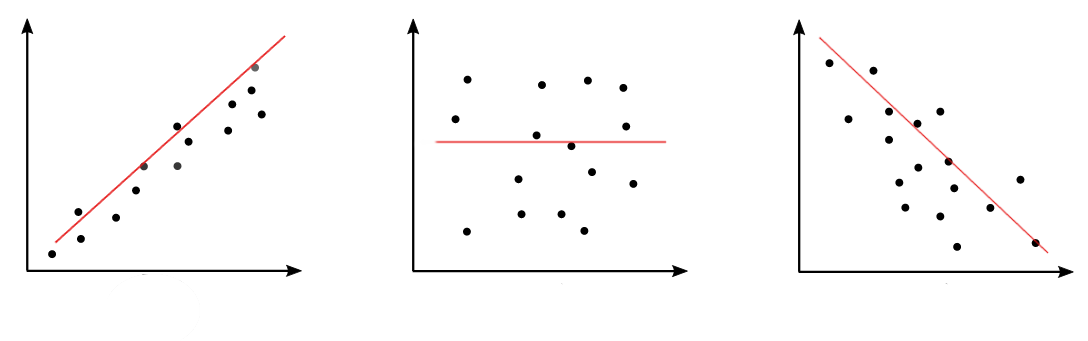
\includegraphics[width=12cm]{pictures/pearson_lines.png}
\caption{Vizualizace lineární korelace dvou náhodných veličin. Směrem zleva zobrazují grafy lineární závislost veličin s hodnotami Pearsonova korelačního koeficientu 0,9; 0 a -0.8.}
\label{PCC_obr}
\end{center}
\end{figure}


